% \chapter{10.12.2010}

\chapter{Die (einseitige) Laplacetransformation}
\Index{Laplace-Transformation}

\begin{definition}
  $f(t)$ sei eine Funktion $f\colon \real_t\to\complex$, und
  $\cn{s}\in\complex$.
  
  Existiert
  \[\int\limits_0^{\infty}|f(t)|\cdot e^{-\Re{\cn{s}}t}\diff t < 0\]
  so heißt $f(t)$ (absolut) $\mathfrak L$-Transformierbar.
  
\end{definition}

  Schreibweise: $\cn{T}(\cn{s}) = \LT{f(t)}(\cn{s})
    := \int\limits_0^\infty f(t)\cdot e^{-\cn{s}t}\diff t$
  
  Die Transformation ist auch für $f\colon \real\to\mathbb{C}$
  gültig und eindeutig,
  wenn man \[f(t)\equiv0 \text{ für } t<0\] vorraussetzt!
  D.h., $f(t)\stackrel{!}{=}\Theta(t)\cdot \tilde{f}(t)$
  
\section{Laplace-ESB}%TODO: sort, extend
\Index{Ersatzschaltbild!Laplace}
\begin{example}\hfill

  \begin{circuitikz}[scale=0.8]
    \draw (0,0) to [C,v_>=$u_c(t)$,i>^=$i_c(t)$,*-*] (3,0);
  \end{circuitikz},
  $u_c(0^+) \stackrel{!}{=} U_{C,0}$, wende auf die ZGL die Laplacetrafo an:
  \begin{align*}
    \LT{i_c(t)}(\cn{s})
      &=\int\limits_0^\infty C\cdot \frac{\partial}{\partial t} u_c(t)
        \cdot e^{-\cn{s}t} \diff t  \\
    \intertext{\centering (Anwendung partielle Integration:
      $\int u'\cdot v = \int( u\cdot v)'- \int u\cdot v'$ ) }
      &=\int\limits_0^\infty \left(C\cdot u_C(t)\cdot e^{-\cn{s} t}\right)'
        - C\cdot u_C(t)\cdot (-\cn{s})\cdot e^{-\cn{s}t}\diff t \\
      &=\left[C\cdot u_C(t)\cdot e^{-\cn{s} t}\right]_0^\infty +\cn{s}C
        \cdot\underbrace{\int\limits_0^\infty u_C(t)\cdot e^{-\cn{s}t}\diff t}_{
          \cn{U}_C(\cn{s})}  \\
      &=-C\cdot u_C(0^+)\cdot 1+\cn{s}C\cdot \cn{U}_C(\cn{s})
  \end{align*}
  Das kann man auch als "`NWM"' aufschreiben (Laplace-ESB):
  
  \begin{minipage}{0.5\textwidth}
    \centering
    \begin{circuitikz}[scale=1.0]
      \draw (0,0)
        to [short, o-, i_<=$\cn{I}_C(\cn{s})$] (1,0)
        to [R=$\cn{s}C$,*-*, v_<=$\cn{U}_C(\cn{s})$] (3,0)
        to [short, -o] (4,0)
        (3,0) -- (3,1.5)
        to [I, i_<=$C\cdot u_c(0^+)$] (1,1.5)
        -- (1,0)
    ;\end{circuitikz}
  \end{minipage}
  \begin{minipage}{0.5\textwidth}
    \[\Rightarrow\quad
      \cn{I}_C(\cn{s}) = \cn{s}C\cdot \cn{U}_C(\cn{s})-C\cdot u_C(0^+)\]
  \end{minipage}
\end{example}

Für die in WuN wichtigen Funktionen findet man die $\mathfrak{L}$-Transformierte
in der Tabelle (siehe FS (Formelsammlung)).

\paragraph{Definition} (wichtig!): Eine ÜF ist definiert durch
\Index{Übertragungsfunktion}
  \[\left.\cn{H}(\cn{s}) := 
    \frac{\cn{A}(\cn{s})}{\cn{E}(\cn{s})}\right|_{\begin{array}{l}
      \text{\footnotesize Alle $AW\stackrel{!}{=}0$}\\
      \text{\footnotesize Alle anderen festen Quellen $\stackrel{!}{=}0$}
    \end{array}}
    \qquad
    \begin{array}{lp{3cm}}
      \cn{A}(\cn{s}): &\text{Ausgang}  \\
      \cn{E}(\cn{s}): &\text{Eingang,}
        \text{häufige eine feste Quelle,}
        \text{kann auch eine beliebige}
        \text{Zweiggöße sein}
    \end{array}\]

  Darf man bei der $\mathfrak{L}$-Trafo auch $\cn{s}=j\omega$ einsetzen
  (NUR bei asympt. stabilen NWM möglich), stimmt 
  $\cn{H}(\cn{s})|_{\cn{s}=j\omega}$ mit dem Frequenzgang überein.
\Index{Frequenzgang}

\paragraph{Stoßantwort}
\Index{Stoßantwort}
  Die Stoßantwort $a_\delta(t)$ auf eine Quelle $e(t)$ erhält man durch
  \[\cn{H}(\cn{s}) := \frac{\cn{A}(\cn{s})}{\cn{E}(\cn{s})},\quad
    \cn{E}(\cn{s}) = \LT{\delta(t)}(\cn{s}) \underset{\text{Tabelle}}{=} 1\]
  \infobox{Berechnung der Stoßantwort (wichtig!)}{
    \[\begin{array}{lccc}
          &\cn{A}(\cn{s})  &= &\cn{H}(\cn{s})\,\cdot\, 1  \\
        \mathfrak{L}^{-1} &\InversTransformVert & &\InversTransformVert  \\
          &a_\delta(t) &= &\mathfrak{L}^{-1}\{\cn{H}(\cn{s})\}(t)
      \end{array}\]}

\section{Der Laplace-Faltungssatz}
\Index{Laplace-Faltungssatz}
  \[\LT{(f(t')\ast g(t'))(t)} = \cn{F}(\cn{s})\cdot\cn{G}(\cn{s})\]

  \begin{minipage}{0.45\textwidth}
  \infobox{Extrem wichtig!}{\vspace{-1em} %TODO: check why hack is needed!
    \[\begin{array}{lccc}
      &\cn{A}(\cn{s}) &= &\cn{H}(\cn{s}) \cdot \cn{E}(\cn{s})  \\
      \mathfrak{L}^{-1}\{\}(t)  & \InversTransformVert & &\InversTransformVert\\
      &a_{rz}(t) &= &(a_\delta(t') \ast e(t'))(t)
    \end{array}\]}
  \end{minipage}
  \hfill
  \begin{minipage}{0.5\textwidth}
  \paragraph{Nebenbedingungen:}
    \begin{tabularx}{\textwidth}{lX}
      $\cn{H}(\cn{s})$:
        & Alle AW$\stackrel{!}{=}0$, \newline
          alle anderen festen Quellen $\stackrel{!}{=}0$ \\
      $\cn{E}(\cn{s})$:
        & $e(t)\stackrel{!}{=}0\text{ für } t<0$
    \end{tabularx}\medskip

    Diese Bedingungen entsprechen gerade der Antwort aus dem \acs{RZ} bei $t=0$.
  \end{minipage}

Für asymptotisch stabile NWM im eingeschwungenen Zustand (AW abgeklungen)
gilt ebenfalls:

  \begin{minipage}{0.45\textwidth}
  \infobox{Extrem wichtig!}{
    \[a_{ez}(t) = (a_\delta(t') \ast e_\infty(t'))(t)\]}
  \end{minipage}
  \hfill
  \begin{minipage}{0.5\textwidth}
    $e_\infty(t)$ muss für $t<0$ beschränkt sein!
    (Durch $e^{-\frac t\tau}$, $\tau >\underset{i}{\operatorname{max}}
      \left\{\frac{-1}{\Re{\cn{A}_i}}\right\}$)
  \end{minipage}

\paragraph{Anwendung}
  \begin{itemize}[label=$\rightarrow$]
    \item Faltung im Zeitbereich:
      \begin{enumerate}[label=\arabic*.)]
        \item $e(t)$ is ein PWL-Signal (Weltformel!), Faltungsrechenregeln
          verwenden!
        \item $e(t)$ ist nicht L-transformierbar (behandelt man in WuN nicht,
          z.B. $e(t) = V\cdot e^{\frac{t^2}{\tau^2}}\Theta(t)$
      \end{enumerate}
    \item Faltung im Laplace-Bereich:
      \begin{itemize}[label=$\rightarrow$]
        \item Alle anderen Fälle
      \end{itemize}
  \end{itemize}


\section{Beispiel: H07 A1}

\begin{center}
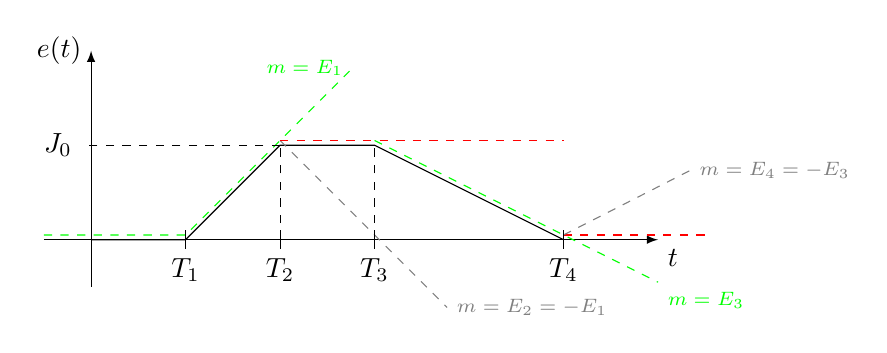
\begin{tikzpicture}[scale=1.2]
  % coords
  \draw[->,>=latex] (-0.5,0) -- (6,0) node [below right] {$t$};
  \draw[->,>=latex] (0,-0.5) -- (0,2) node [left] {$e(t)$};
  % function
  \draw (0,0) -- ++(1,0) -- ++(1,1) -- ++(1,0) -- ++(2,-1);
  % help functions
  \draw[dashed, green] (-0.5,0.05) -- ++(1.5,0) -- ++(45:2.5) node[left] {\scriptsize $m=E_1$};
  \draw[dashed, gray] (2,1.05) -- ++(-45:2.5) node[right] {\scriptsize $m=E_2=-E_1$};
  \draw[dashed, red] (2,1.05) -- ++(3,0);
  \draw[dashed, green] (3,1.05) -- ++(3,-1.5) node[below right] {\scriptsize $m=E_3$};
  \draw[dashed, red] (5,0.05) -- ++(1.5,0);
  \draw[dashed, gray] (5,0.05) -- ++(27:1.5) node[right] {\scriptsize $m=E_4=-E_3$};
  % time
  \draw (1,0.1) -- +(0,-0.2) node [below] {$T_1$};
  \draw (2,0.1) -- +(0,-0.2) node [below] {$T_2$};
  \draw[dashed] (2,0) -- ++(0,1);
  \draw (3,0.1) -- +(0,-0.2) node [below] {$T_3$};
  \draw[dashed] (3,0) -- ++(0,1);
  \draw (5,0.1) -- +(0,-0.2) node [below] {$T_4$};
  % J0
  \draw[dashed] (2,1) -- ++(-2.1,0) node [left] {$J_0$};
\end{tikzpicture}
\end{center}
% 
\begin{align*}
  j(t) &= \;\; \underbrace{\left(\frac{J_0}{T_2-T_1}\right)}_{E_1}
    \cdot(t-T_1) \cdot\Theta(t-T_1)
  + \underbrace{\left(-\frac{J_0}{T_2-T_1}\right)}_{E_2}
    \cdot(t-T_2) \cdot\Theta(t-T_2)\\
  &\;\; + \underbrace{\left(-\frac{J_0}{T_4-T_3}\right)}_{E_3}
    \cdot(t-T_3) \cdot\Theta(t-T_3)
  + \underbrace{\left(\frac{J_0}{T_4-T_3}\right)}_{E_4}
    \cdot(t-T_4) \cdot\Theta(t-T_4) \\
  &= \sum_{k=1}^{4} E_k\cdot \Theta(t-T_k)\cdot(t-t_k)
\end{align*}

\paragraph{Verschiebungssatz}
\[\left(e(t'{\color{blue}-\tau})\ast a_g(t')\right)(t)
  = \left(e(t')\ast a_g(t')\right)(t{\color{blue}-\tau})\]



\section{Beispiel: H08 A1 e)}

\acs{ESB} im Laplace-Bereich (\acs{AW}$\stackrel{!}{=}0$):

\begin{minipage}{0.5\textwidth}
\begin{circuitikz}
  \draw (0,0) 
    -- (0,1)
    to[I=$\cn{J}(\cn{s})$] (0,3)
    -- (0,4)
    -- (2,4)
    to[R=$R$] (4,4)
    to[short,i=$\cn{I}_2(\cn{s})$] (4,0)
    -- (0,0)
    (2,4)
    to[C=$C$,*-] (2,2)
    to[R=$R$,-*] (2,0)
;\end{circuitikz}
\end{minipage}
\begin{minipage}{0.5\textwidth}
\begin{align*}
  \cn{H}(\cn{s})
    &=\frac{\cn{I}_L(\cn{s})}{\cn{J}(\cn{s})} \\
    &=\frac{R+\frac{1}{\cn{s}C}}{\left(R+\frac{1}{\cn{s}C}\right)+R}  \\
    &=\frac{\cn{s}RC+1}{\cn{s}2RC+1}  \\
    &=\frac{RC}{2RC}\cdot\frac{\cn{s}+\frac{1}{RC}}{\cn{s}+\frac{1}{2RC}} \\
    &=\frac{1}{2}\left(\frac{\cn{s}+\frac{1}{2RC}-\frac{1}{2RC}+\frac{1}{RC}}
      {\cn{s}+\frac{1}{2RC}}\right) \\
    &=\frac{1}{2}\left(1+\frac{1}{2RC}\cdot\frac{1}{\cn{s}+\frac{1}{2RC}}\right)
\end{align*}
\end{minipage}

\begin{enumerate}
  \item Antwort aus dem \acs{RZ}? \\
    (oder) Antwort im EZ? \\
    (oder) ``zero-state''-response berechnen?

    Wenn ja: Faltung!

    Hier: kein \acs{AW}, $j(t)=0$ für $t<T_1 \Rightarrow$AW aus dem \acs{RZ}!
  \item
    \colorbox{blue!20}{
    \begin{minipage}{0.6\textwidth}
    \[e(t) =\underbrace{\sum_{k=1}^{n} E_k
          \cdot\Theta(t-T_k)\cdot(t-T_k)}_{
            \text{Knick-Funktionen}}
        +\underbrace{\sum_{k=1}^{n}F_k\Theta(t-T_k)}_{\text{Sprünge} }
    \]
    \end{minipage}}
    \hfill
    \begin{minipage}{0.3\textwidth}
            \footnotesize allgemeine Fkt.-Gleichung eines \acs{PWL}-Signals,
            nur für diese funktioniert die ``Welt-Formel''!
    \end{minipage}
  
  \begin{minipage}{0.3\textwidth}
  \begin{tikzpicture}
    % coords
    \draw[->,>=latex] (-0.5,0) -- (4,0) node [below right] {$t$};
    \draw[->,>=latex] (0,-0.5) -- (0,2) node [left] {$j(t)$};
    % function
    \draw[blue] (0,0) -- (1,0);
    \draw[dashed,blue] (1,0) -- (1,1);
    \draw[blue] (1,1) -- (2,1) -- (3,0) -- (4,0);
    % time
    \draw (1,0.1) -- +(0,-0.2) node [below] {$T_1$};
    \draw (2,0.1) -- +(0,-0.2) node [below] {$2T_1$};
    \draw (3,0.1) -- +(0,-0.2) node [below] {$3T_1$};
    % J0
    \draw[dashed] (0.1,1) -- ++(-0.2,0) node [left] {$J_0$};
  \end{tikzpicture}
  \end{minipage}%
  \begin{minipage}{0.7\textwidth}
    \begin{align*}
      e(t) &=\underbrace{(J_0-0)\cdot\Theta(t-T_1)}_{
          E_1:=0,\, F_1:=J_0}\\
        &\;\;\;+\underbrace{\left(-0+\frac{0-J_0}{3T_1-2T_1}\right)
          \cdot\Theta(t-2T_1)\cdot(t-2T_1)}_{
            E_2:=-\frac{J_0}{T_1},\, F_2:=0,\, T_2:=2T_1}\\
        &\;\;\;+\underbrace{\left(-\frac{0-J_0}{3T_1-2T_1}+0\right)
          \cdot\Theta(t-3T_1)\cdot(t-3T_1)}_{
            E_3:=-\frac{J_0}{T_1},\, F_3:=0,\, T_3:=3T_1}  \\
      &=\sum_{k=1}^{3} E_k\Theta(t-T_k)\cdot(t-T_K)
        +\sum_{k=1}^{3} F_k\Theta(t-T_k)
    \end{align*}
  \end{minipage}


  \item Bestimmung der Stoßantwort mittels inverser Laplace-Transformation
    \[a_\delta(t) = \mathfrak{L}^{-1}\{\cn{H}(\cn{s})\}(t)\]
    % 
    \[\begin{array}{lccll}
      &\cn{H}(\cn{s})
        &= &\frac{1}{2}&+\dfrac{1}{4RC}\cdot\dfrac{1}{\cn{s}+\frac{1}{2RC}}\\
      \mathfrak{L}^{-1} &\InversTransformVert & 
        &\InversTransformVert&\qquad\qquad\InversTransformVert  \\
      &a_\delta(t) &= &\frac{1}{2}\delta(t) 
        &+ \dfrac{1}{4RC}\cdot\left[\Theta(t)\cdot e^{-\frac{t}{2RC}}\right]
        \quad\leftarrow\text{Distributionsklammern}
    \end{array}\]

\end{enumerate}

